\chapter{Υλοποίηση συστήματος Μηχανικής Μάθησης}

Αυτό το κεφάλαιο περιγράφει την διαδικασία σχεδιασμού και υλοποίησης των μοντέλων που αναπτύχθηκαν με σκοπό την παραγωγή επιπέδων, παρόμοιων χαρακτηριστικών, με τα επίπεδα που αναλύθηκαν στον κεφάλαιο 2. Η υλοποίηση είναι μια εφαρμογή Machine Learning Content Generation (MLCG). Αποτελεί μια απόδειξη, από την θεωρία στην πράξη της υπόθεσης ότι μοντέλα Deep Neural Networks και συγκεκριμένα GANs μπορούν να χρησιμοποιηθούν με επιτυχία για την κατασκευή περιεχομένου.
\par
Η υλοποίηση περιλάμβανε την ολοκλήρωση πολλών επιμέρους κομματιών, κάποια από τα οποία δεν χρησιμοποιήθηκαν τελικά στην εκπαίδευση του τελικού μοντέλου. Κάτι το οποίο είναι συχνό και αναμενόμενο όταν υλοποιούνται εφαρμογές τέτοιας πολυπλοκότητας. Για παράδειγμα υλοποιήθηκαν μέθοδοι που πρόσθεταν θόρυβο στις διακριτές τιμές της εισόδου ώστε να μετατρέπονται σε συνεχείς τιμές με κανονική κατανομή. Αυτό το κομμάτι αποδείχθηκε ότι τελικά δεν προσφέρει στην απόδοση του συστήματος οπότε δεν χρησιμοποιείται στα τελικά αποτελέσματα, που θα αναλυθούν. Παραμένει κομμάτι της υλοποίησης χωρίς όμως να συνεισφέρει στο τελικό αποτέλεσμα.

\section{Τεχνική περιγραφή}
Το σύστημα MLCG αναπτύχθηκε στην γλώσσα\textit{Python}, μια από τις πιο διαδεδομένες γλώσσες για υλοποιήσεις Μηχανικής Μάθησης. Η έκδοση που χρησιμοποιήθηκε είναι η 3.7. Επιλέχθηκε η συγκεκριμένη έκδοση καθώς είναι η πιο πρόσφατη έκδοση της γλώσσας, που υποστηρίζει τις βιβλιοθήκες για Deep Neural Networks που χρησιμοποιήθηκαν. 
Μερικές από τις πιο σημαντικές βιβλιοθήκες και εργαλεία που χρησιμοποιήθηκαν:

\begin{description}
\item[$\bullet$ Numpy] Βιβλιοθήκη για επιστημονικές εφαρμογές και υπολογισμούς της γλώσσας Python.
\item[$\bullet$ Matplotlib] Βιβλιοθήκη για την οπτικοποίηση αποτελεσμάτων και μετρικών.
\item[$\bullet$ Tensorflow] Αποτελεί ένα ολοκληρωμένο σύστημα για εφαρμογές Machine Learning με υποστήριξη για πολλές γλώσσες προγραμματισμού. 
\item[$\bullet$ Keras] Αποτελεί την βιβλιοθήκη σε Python, για την χρησιμοποίηση του συστήματος Tensorflow σε εφαρμογές ανεπτυγμένες σε αυτή την γλώσσα.
\item[$\bullet$ Tensorboard] Μια βιβλιοθήκη οπτικοποίησης των αποτελεσμάτων εκπαίδευσης και αρχιτεκτονικής που χρησιμοποιείται σε συνδυασμό με την βιβλιοθήκη \textit{Tensorflow}. 
\end{description}


\section{Δεδομένα εκπαίδευσης}
Όπως αναλύθηκε και στο κεφάλαιο σχετικά με την υλοποίηση του PCG συστήματος σε Python, το dataset αποτελείται από αρχεία κειμένου, όπου το κάθε αρχείο αντιστοιχεί σε ένα επίπεδο. Για την εκπαίδευση του μοντέλου, δημιουργήθηκε ένα \textit{dataset} που περιλαμβάνει 1000 τέτοια αρχεία.
\par
Όπως σε όλες τις εφαρμογές Μηχανικής Μάθησης, τα δεδομένα του dataset δεν δίνονται απευθείας στο μοντέλο για εκπαίδευση αλλά περνάνε από διάφορες μεθόδους προεργασίας ώστε να εξασφαλίσουμε καλύτερα και πιο αξιόπιστα αποτελέσματα.


\subsection{Χαρακτηριστικά του dataset}
Το κάθε επίπεδο είναι ένας πίνακας \textit{10000} στοιχείων, όπου το κάθε στοιχείο αντιστοιχεί σε ένα κελί στην 100x100 grid απεικόνιση του επιπέδου. Μόλις το PCG σύστημα δημιουργεί ένα επίπεδο, το μετατρέπει στην αναπαράσταση του αρχείου και το αποθηκεύει ώστε να μπορεί να διαβαστεί από το σύστημα Μηχανικής Μάθησης.
\par
Απόσπασμα από αρχείο του dataset:
\begin{verbatim}
30, 30
Tile X,Tile Y,Tile Type
0,0,1
0,1,1
0,2,1
0,3,1
0,4,1
0,5,1
\end{verbatim}
Στο παραπάνω παράδειγμα βλέπουμε τις πρώτες γραμμές από ένα αρχείο επιπέδου. Η πρώτη σειρά δηλώνει το μέγεθος του επιπέδου, κάτι το οποίο προστέθηκε για πληροφοριακούς λόγους αλλά δεν χρησιμοποιείται από το MLCG. Η δεύτερη σειρά αναγράφει το είδος των στοιχείων που αντιστοιχούν στην κάθε κολόνα αντίστοιχα.
\par

\begin{itemize}
\item Η πρώτη κολόνα, Tile X, δηλώνει την x συντεταγμένη του στοιχείου μέσα στο επίπεδο.
\item Η δεύτερη κολόνα, Tile Y, δηλώνει την y συντεταγμένη του στοιχείου μέσα στο επίπεδο.
\item Η τρίτη κολόνα, Tile Type, δηλώνει το είδος του στοιχείου \textit{(Wall, Room)} με ένα διακριτό ακέραιο αριθμό αντίστοιχα.
\end{itemize}

\par
H αρίθμηση των στοιχείων μέσα στο grid ξεκινάει από την κάτω αριστερή γωνία, αυτό είναι το στοιχείο με συντεταγμένες 0,0 και προχωράει πρώτα στον κάθετο άξονα (Υ) και στη συνέχεια στον οριζόντιο άξονα (Χ). Το τελευταίο στοιχείο που αναγράφετε με συντεταγμένες 29,29 αντιστοιχεί στην πάνω δεξιά γωνία του grid.

\subsection{Προ επεξεργασία Δεδομένων}
Πριν από το στάδιο της εκπαίδευσης, τα δεδομένα που θα εισάγουμε στο σύστημα πρέπει να περάσουν από το στάδιο της προ επεξεργασίας ώστε να πληρούν κάποιες προϋποθέσεις.
\par
Σε αυτή την εφαρμογή έχουμε δύο ειδών τιμές που μπορεί να λάβει ένα στοιχείο \textit{(Wall, Room)} τα οποία είναι αντίστοιχα οι αριθμοί \textit{(0, 1)}. Ως προ επεξεργασία των δεδομένων εφαρμόζετε \textit{One hot encoding} στα δεδομένα μας το οποίο λαμβάνει μια διακριτή τιμή και την μετατρέπει σε ένα διάνυσμα τιμών. Το διάνυσμα αυτό έχει ένα \textit{1} και όλα τα υπόλοιπα στοιχεία \textit{0}.
\par
Για παράδειγμα, στην περίπτωση της εφαρμογής το στοιχείο με αριθμό \textit{0} θα μετατραπεί στο διάνυσμα \textit{(1, 0)} και αντίστοιχα το στοιχείο  με αριθμό \textit{1} θα μετατραπεί στο διάνυσμα \textit{(0, 1)}. 
\par
To \textit{One hot encoding} συνίσταται σε εφαρμογές που δεν έχουν πολλές διακριτές τιμές τα δεδομένα τους, όπως σε αυτή την εφαρμογή.

\par
Το δεύτερο κομμάτι αφορά το είδος του μοντέλου που θέλουμε να εκπαιδεύσουμε. Στην υλοποίηση της εργασίας αναπτύχθηκε ένα μοντέλο GAN, το Convolutional επειδή αποτελείται κυρίως από επίπεδα συνέλιξης (\textit{convolution}). Το μοντέλο ανάλογα με τα επιπέδων που έχει, δέχεται την είσοδο σε διαφορετική μορφή από αυτήν στην οποία είναι αποθηκευμένα τα επίπεδα. Το Convolutional μοντέλο δέχεται ως είσοδο ένα διάνυσμα (100, 1) αριθμών και παράγει ως έξοδο ένα πίνακα (100, 100) στοιχείων.
\par


\section{Επεξεργασία Αποτελεσμάτων}
Η αντίθετη διαδικασία πρέπει να εκτελεστεί για τα αποτελέσματα του μοντέλου GAN. Τα αποτελέσματα του Convolutional μοντέλου πρέπει να μετατραπούν σε διάνυσμα (900, 1) για να αποθηκευτούν με την μορφή που έχει όλο το dataset.
\par
Επίσης τα αποτελέσματα είναι σε \textit{One hot encoding} αναπαράσταση και πρέπει να γίνει η μετατροπή τους αντίστοιχη διακριτή τιμή από τις διαθέσιμες [0, 1]. Τα αποτελέσματα του Gan δεν είναι σε απόλυτες τιμές (0, 1) ακόμα και στην \textit{One hot encoding} αναπαράσταση, αλλά έχουν τις τιμές των πιθανοτήτων που προέβλεψε το μοντέλο για το κάθε στοιχείο του διανύσματος. 
\par
Για παράδειγμα μπορεί ένα στοιχείο να προβλεφτεί από το μοντέλο ως \textit{(0.6, 0.4)}, σε αυτή την περίπτωση μετατρέπουμε την μεγαλύτερη πιθανότητα σε \textit{(1)} και όλες τις υπόλοιπες σε \textit{(0)}. Συνεπώς το παράδειγμα θα γίνει \textit{(1, 0)} το οποίο αντίστοιχα θα μεταφραστεί ως \textit{(0)} με βάση την αντιστροφή της αρχικής διαδικασίας του \textit{One hot encoding}.


\subsection{Δειγματοληψία κατά την εκπαίδευση}
Για να παρακολουθούμε την πρόοδο της εκπαίδευσης ανά τακτές χρονικές περιόδους, ορίστηκε μια μεταβλητή που δηλώνει ανά πόσες εποχές, θα γίνετε δειγματοληψία από το μοντέλο. Επίσης μια τελική δειγματοληψία γίνετε μόλις ολοκληρωθούν όλες οι εποχές της εκπαίδευσης ώστε να έχουμε δείγμα από το τελικό μοντέλο. 
\par
Σε κάθε δειγματοληψία, το μοντέλο εκτελείται με μια είσοδο εκπαίδευσης και με βάση τα βάρη που έχει εκείνη την στιγμή. Το αποτέλεσμα περνάει από την επεξεργασία που αναλύθηκε παραπάνω και αποθηκεύεται σε ένα αρχείο με όνομα που να εκφράζει το στάδιο της εκπαίδευσης στο οποίο βρισκόταν το νευρωνικό όταν δημιουργήθηκε αυτό το δείγμα.
\par
Για παράδειγμα το αρχείο \verb|combined_1000_09-03-2020_21-11-56FGAE.csv| είναι ένα δείγμα που δημιουργήθηκε από τον Generator σε συνεργασία με τον Discriminator (\textit{combined}) στην εποχή 1000 της εκπαίδευσης. Τα υπόλοιπα στοιχεία δηλώνουν την ημερομηνία που εκτελέστηκε η συγκεκριμένη εκπαίδευση. Στο τέλος του κάθε ονόματος προστίθεται και ένα τυχαίο αλφαριθμητικό. 
\par
Το μοντέλο που δημιούργησε αυτό το δείγμα αναφέρεται στον φάκελο που είναι αποθηκευμένο \verb|cnn_gan-09_03_2020_21_08_34|. Αυτή η ονοματολογία δηλώνει ότι είναι το Convolutional μοντέλο (\textit{cnn} και στην συνέχεια ακολουθεί η ημερομηνία και η ώρα που ξεκίνησε η εκπαίδευση του συγκεκριμένου μοντέλου.

\subsection{Αποθήκευση μοντέλου}
Το κάθε μοντέλο μόλις εκπαιδευτεί, αποθηκεύεται σε αρχεία από τα οποία είναι δυνατή η φόρτωση του στην κατάσταση που ήταν μόλις τελείωσε η εκπαίδευση. Συγκεκριμένα αποθηκεύεται η αρχιτεκτονική και τα βάρη του μοντέλου, σε ειδικά αρχεία ώστε να μπορούμε οποιαδήποτε στιγμή να τα φορτώσουμε και να τα εκτελέσουμε. Η αποθήκευση γίνεται μέσα στον φάκελο του μοντέλου, που δημιουργείται μόλις ξεκινήσει η εκπαίδευση.
\par
Μέσα στον φάκελο του μοντέλου αποθηκεύονται:
\begin{description}
\item[$\bullet$ Χαρακτηριστικά του μοντέλου] Όλη η αρχιτεκτονική του μοντέλου, τα επίπεδα, ο αριθμός και το είδος των παραμέτρων του κάθε επιπέδου, για το δίκτυο του Generator και του Discriminator. Αυτά αποθηκεύονται μέσα στον φάκελο \texttt{model\_data} στα αρχεία  \textit{generator.json} και \textit{discriminator.json} αντίστοιχα.
\item[$\bullet$ Τα βάρη του μοντέλου] Σε αντίστοιχα αρχεία \textit{generator.h5} και \textit{discriminator.h5} αποθηκεύονται τα βάρη του κάθε δικτύου.
\item[$\bullet$ Μετρικές και αποτελέσματα] Στο αρχείο \textit{results.txt} αποθηκεύονται οι τελικές μετρήσεις και αποτελέσματα της απόδοσης του κάθε μοντέλου μαζί με διάφορες παραμέτρους που έχουμε ορίσει για την εκπαίδευση και τις τιμές τους. Με αυτό τον τρόπο μπορούμε εύκολα να συγκρίνουμε τα διάφορα μοντέλα.
\item[$\bullet$ Επίπεδα που παράχθηκαν] Στον φάκελο \textit{Results} αποθηκεύονται τα επίπεδα που δημιουργήθηκαν με την δειγματοληψία που αναφέραμε παραπάνω.
\item[$\bullet$ Εικόνες επιπέδων] Τα επίπεδα που δημιουργούνται μέσω της δειγματοληψίας, αποτυπώνονται και σε εικόνες για την άμεση παρακολούθηση και αξιολόγηση της εκπαίδευσης όσο εκτελείται και για την σύγκριση αποτελεσμάτων μεταξύ εκπαιδεύσεων. Αυτές οι εικόνες αποθηκεύονται στον φάκελο \textit{Images} του κάθε μοντέλου.
\item[$\bullet$ Αρχεία Tensorboard] Τα αρχεία με τα αποτελέσματα της εκπαίδευσης, και την αρχιτεκτονική των μοντέλων τα οποία μπορούν να χρησιμοποιηθούν από την βιβλιοθήκη του Tensorboard, αποθηκεύονται στον φάκελο \textit{com\_logs}. Από αυτά τα αρχεία μπορούν να παραχθούν γραφήματα και μετρικές σχετικά με την πρόοδο του μοντέλου.
\end{description}


Το μοντέλο GAN που αναφέρεται ως Dense είναι το πρώτο μοντέλο GAN που αναπτύχθηκε και εκπαιδεύτηκε στα πλαίσια αυτής της εργασίας. Αναφέρεται σε διάφορα παραδείγματα υλοποιήσεων GAN \cite{firstgan3} \cite{firstgan} \cite{firstgan2} και είναι πιο εύκολο στην κατανόηση και υλοποίηση. Αναφέρεται ως μοντέλο Dense επειδή η επεξεργασία των εισόδων γίνετε στα Dense επίπεδα του δικτύου.

\subsection{Αρχιτεκτονική Generator}
Το μοντέλο του Generator δικτύου, αποτελείται από 22 επίπεδα συνολικά, από τα οποία τα πρώτα 21 μπορούν να χωριστούν σε τριάδες καθώς ακολουθούν μια κοινή αρχιτεκτονική και το τελευταίο επίπεδο δημιουργεί την έξοδο με τις διαστάσεις του επιπέδου όπως τις έχουμε ορίσει. Κάθε τριάδα επιπέδου ξεκινάει με ένα Dense επίπεδο, στην συνέχεια υπάρχει ένα LeakyReLU επίπεδο \cite{leakyrelu} και το τρίτο επίπεδο εναλλάσσετε από BatchNormalization επίπεδο σε Dropout. 

\begin{description}
\item[$\bullet$ Dense επίπεδο] Το κάθε Dense επίπεδο, πέρα από το αρχικό που λαμβάνει ως είσοδο το επίπεδο ως διάνυσμα (900, 1) στοιχείων, παίρνει ως είσοδο, την έξοδο του προηγούμενου επιπέδου. Για κάθε Dense επίπεδο ορίζουμε τον αριθμό των \textit{units} που θα έχει ως έξοδο. Για παράδειγμα για το επίπεδο εισόδου ορίζουμε:
\begin{verbatim}
Dense(units=256, input_dim=self.dungeon_dimension)
\end{verbatim}
\par
Το παραπάνω επίπεδο έχει είσοδο ένα διάνυσμα (900, 1) και ως έξοδο ένα διάνυσμα (256, 1). Το μέγεθος της εισόδου πρέπει να καθοριστεί μόνο στο αρχικό επίπεδο του δικτύου, τα επόμενα επίπεδα γνωρίζουν τι είσοδο δέχονται με βάση την έξοδο του προηγούμενου επιπέδου.  \cite{dense}
\end{description}

\begin{description}
\item[$\bullet$ LeakyReLU] Μετά από κάθε Dense επίπεδο στην κάθε τριάδα, υπάρχει ένα επίπεδο \textit{LeakyReLU}. Αυτό το επίπεδο είναι μια παραλλαγή του επιπέδου \textit{ReLU} που αναλύσαμε. Η διαφορά  του επιπέδου LeakyReLU είναι ότι στην περίπτωση μη ενεργοποίησης του επιπέδου από την είσοδο, η έξοδος δεν είναι μηδενική όπως στο επίπεδο της \textit{ReLU} αλλά επιστρέφει ως έξοδο μια πολύ μικρή τιμή, γιαυτό και λέγεται \textit{LeakyReLU}(διαρροή). Η συνάρτηση ενεργοποίησης της LeakyReLU ορίζετε ως:
\par
$f(x) = alpha * x,  \;\; if \;\; x < 0$
\par
$f(x) = x,  \;\; if \;\; x >= 0$
\par
To alpha είναι μια παράμετρος που μπορεί να οριστεί σε κάθε επίπεδο LeakyReLU. Στην συγκεκριμένη υλοποίηση ορίστηκε ως εξής:
\begin{verbatim}
LeakyReLU(alpha=0.2)
\end{verbatim}
\par
O ορισμός του alpha με την τιμή 0.2 έγινε μετά από έρευνα σε αντίστοιχες υλοποιήσεις και παρατηρήσεις κατά την εκπαίδευση. \cite{firstgan} \cite{firstgan2} \cite{firstgan3} 
\end{description}

\begin{description}
\item[$\bullet$ BatchNormalization] To τελευταίο επίπεδο σε κάθε τριάδα, είναι είτε το επίπεδο του BatchNormalization, ή το επίπεδο Dropout. To επίπεδο του BatchNormalization όπως αναφέρει και το όνομα κανονικοποιεί την είσοδο που δέχεται. To επίπεδο Dropout απενεργοποιεί τυχαία κάποιες από τις εξόδους μετατρέποντας τις τιμές τους σε 0.
\par
\begin{verbatim}
BatchNormalization(momentum=0.8)
Dropout(rate=0.3)
\end{verbatim}
\par
Η παράμετρος momentum χρησιμοποιείται με την τιμή 0.8 για να βελτιώσει την απόδοση του νευρωνικού και να αυξήσει την ταχύτητα της εκπαίδευσης \cite{firstgan}. 
\par
H παράμετρος rate δηλώνει το ποσοστό επί τις εκατό των τιμών που θα γίνουν 0 στο επίπεδο Dropout.
\end{description}

\begin{description}
\item[$\bullet$ Dense επίπεδο εξόδου] To τελευταίο επίπεδο έχει ως έξοδο το διάνυσμα του παραγομένου επιπέδου στις διαστάσεις που το έχουμε ορίσει:
\par
\begin{verbatim}
Dense(np.prod(self.dungeon_shape), activation="tanh")
\end{verbatim}
\par
Σε αντίθεση με τα υπόλοιπα επίπεδα Dense που έχουν την γραμμική συνάρτηση ως συνάρτηση ενεργοποίησης, το συγκεκριμένο επίπεδο έχει την υπερβολική εφαπτομένη για να πάρουμε έξοδο στο πεδίο τιμών [-1, 1] που είναι το πεδίο τιμών που έχουμε ορίσει για τις τιμές του επιπέδου κατά την περίοδο της εκπαίδευσης.
\end{description}

\par
Αρχιτεκτονική μοντέλου:
\begin{verbatim}
Dense(units=256, input_dim=self.dungeon_dimension)
LeakyReLU(alpha=0.2)
BatchNormalization(momentum=0.8)

Dense(units=512)
LeakyReLU(alpha=0.2)
Dropout(rate=0.3)

Dense(units=1024)
LeakyReLU(alpha=0.2)
BatchNormalization(momentum=0.8)

Dense(units=1024)
LeakyReLU(alpha=0.2)
Dropout(rate=0.3)

Dense(units=1024)
LeakyReLU(alpha=0.2)
BatchNormalization(momentum=0.8)

Dense(units=1024)
LeakyReLU(alpha=0.2)
Dropout(rate=0.3)

Dense(units=1024)
LeakyReLU(alpha=0.2)
BatchNormalization(momentum=0.8)

Dense(np.prod(self.dungeon_shape), activation="tanh")
\end{verbatim}

\begin{figure}[H]
\centering
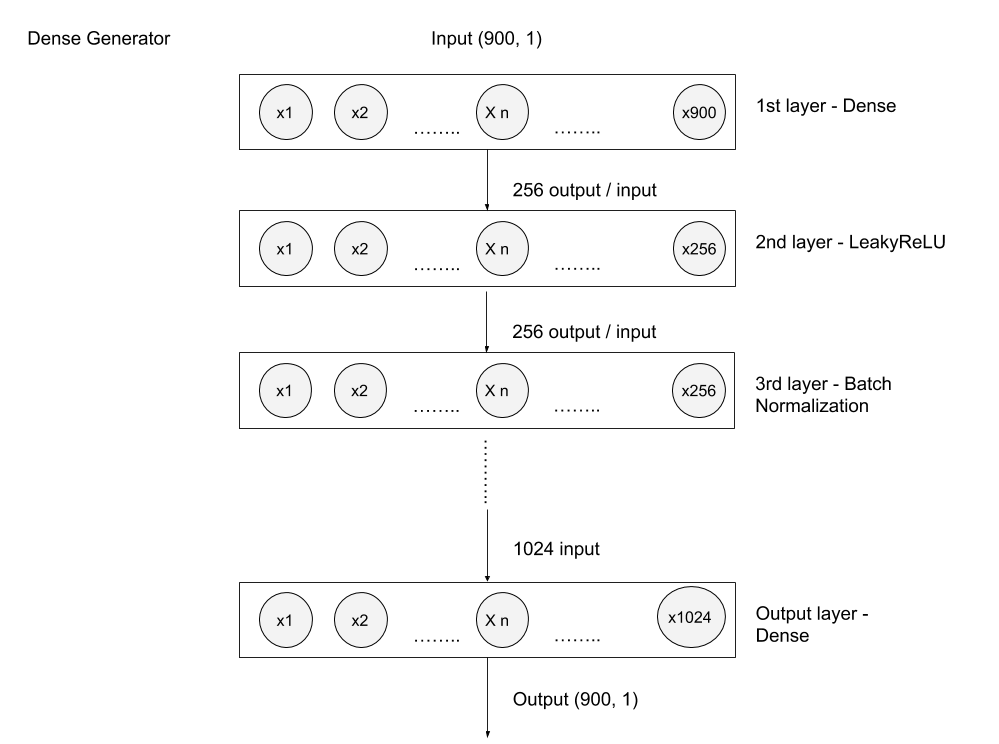
\includegraphics[width=.8\linewidth]{../images/graphs/Dense_generator.png}
\caption{Απεικόνιση των επιπέδων του Dense Generator}
\label{fig:fig}
\end{figure}


\subsection{Αρχιτεκτονική Discriminator}
Το μοντέλο του Discriminator δικτύου, είναι πολύ πιο μικρό από το μοντέλο του Generator. Αποτελείται από μόλις 5 επίπεδα στην τελική του μορφή. Έγιναν και κάποιες δοκιμές με δύο επιπλέον επίπεδα Dropout αλλά στη συνέχεια αφαιρέθηκαν. Η είσοδος του δικτύου είναι ένα επίπεδο διανυσματικής μορφής με τις διαστάσεις και τις τιμές όπως τις έχουμε αναλύσει και έχει ως έξοδο μία τιμή στο διακριτό διάστημα [0, 1].
\par
Τα επίπεδα του Discriminator όπως ορίζονται στην υλοποίηση:
\begin{verbatim}
Dense(units=512, input_dim=self.dungeon_dimension)
LeakyReLU(alpha=0.2)
Dense(units=256)
LeakyReLU(alpha=0.2)
Dense(1, input_dim=self.dungeon_dimension, activation="sigmoid")
\end{verbatim}

\begin{figure}[H]
\centering
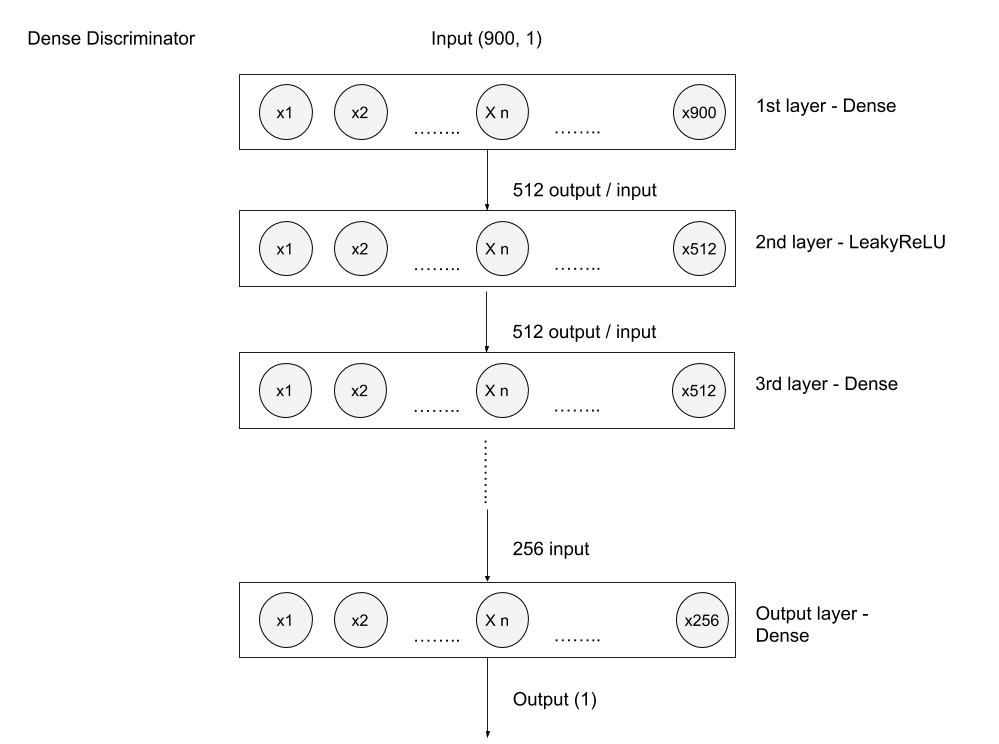
\includegraphics[width=.8\linewidth]{../images/graphs/Dense_discriminator.png}
\caption{Απεικόνιση των επιπέδων του Dense Discriminator}
\label{fig:fig}
\end{figure}

\par
Μπορούμε να διακρίνουμε μια παρόμοια αρχιτεκτονική με τον Generator, έχουμε αρχικά ένα Dense επίπεδο και στη συνέχεια ένα επίπεδο LeakyReLU. Στον Discriminator παρόλαυτα δεν υπάρχει το επίπεδο του BatchNormalization καθώς δεν χρειάζεται να κρατήσουμε τις τιμές των εξόδων σε ένα συγκεκριμένο διάστημα.
\par
To επίπεδο της εξόδου παράγει μία τιμή με συνάρτηση ενεργοποίησης την σιγμοειδή (\textit{sigmoid}) συνάρτηση, ώστε να έχουμε το αποτέλεσμα μεταξύ 0 και 1. Όπου το 0 και τιμές κοντά στο 0 δηλώνουν ότι το επίπεδο αποτελεί δημιούργημα του Generator και όχι κάποιο από τα δείγματα εκπαίδευσης και το 1 δηλώνει ότι το επίπεδο είναι από τα δείγματα εκπαίδευσης ή μοιάζει τόσο πολύ που δεν μπορεί να το ξεχωρίσει από τα "πραγματικά".

\section{Μοντέλο CNN GAN}

Το μοντέλο GAN που αναφέρετε ως CNN είναι το μοντέλο GAN που αναπτύχθηκε και εκπαιδεύτηκε στα πλαίσια αυτής της εργασίας. Η σχεδίαση και ανάπτυξη του βασίστηκε σε Convolutional GAN για δημιουργία χειρόγραφων ψηφίων από το dataset της MNIST \cite{mnist}. 
\par
Αν και ο στόχος της εργασίας δεν είναι ο ίδιος με τον στόχο του παραπάνω GAN, πολλά στοιχεία είναι κοινά, συνεπώς χρησιμοποιήσαμε κομμάτια από την αρχιτεκτονική του για να δημιουργήσουμε το αντίστοιχο CNN GAN δημιουργίας περιεχομένου.

\subsection Περιγραφή επιπέδων
Θα αναλύσουμε περιληπτικά την χρήση του κάθε επιπέδου που χρησιμοποιήθηκε στο μοντέλο GAN.

\begin{description}
\item[$\bullet$ BatchNormalization] To επίπεδο του BatchNormalization όπως αναφέρει και το όνομα κανονικοποιεί την είσοδο που δέχεται.
\par
\begin{verbatim}
BatchNormalization(momentum=0.8)
\end{verbatim}
\par
Η παράμετρος momentum χρησιμοποιείται με την τιμή 0.8 για να βελτιώσει την απόδοση του νευρωνικού και να αυξήσει την ταχύτητα της εκπαίδευσης \cite{firstgan}.
\end{description}

\begin{description}
\item[$\bullet$ Dropout] To επίπεδο Dropout απενεργοποιεί τυχαία κάποιες από τις εξόδους μετατρέποντας τις τιμές τους σε 0.
\par
\begin{verbatim}
Dropout(rate=0.3)
\end{verbatim}. 
\par
H παράμετρος rate δηλώνει το ποσοστό επί τις εκατό των τιμών που θα γίνουν 0 στο επίπεδο Dropout.
\end{description}

\begin{description}
\item[$\bullet$ LeakyReLU] Αυτό το επίπεδο είναι μια παραλλαγή του επιπέδου \textit{ReLU} που αναλύσαμε. Η διαφορά  του επιπέδου LeakyReLU είναι ότι στην περίπτωση μη ενεργοποίησης του επιπέδου από την είσοδο, η έξοδος δεν είναι μηδενική όπως στο επίπεδο της \textit{ReLU} αλλά επιστρέφει ως έξοδο μια πολύ μικρή τιμή, γιαυτό και λέγεται \textit{LeakyReLU}(διαρροή). Η συνάρτηση ενεργοποίησης της LeakyReLU ορίζετε ως:
\par
$f(x) = alpha * x,  \;\; if \;\; x < 0$
\par
$f(x) = x,  \;\; if \;\; x >= 0$
\par
To alpha είναι μια παράμετρος που μπορεί να οριστεί σε κάθε επίπεδο LeakyReLU. Στην συγκεκριμένη υλοποίηση ορίστηκε ως εξής:
\begin{verbatim}
LeakyReLU(alpha=0.2)
\end{verbatim}
\par
O ορισμός του alpha με την τιμή 0.2 έγινε μετά από έρευνα σε αντίστοιχες υλοποιήσεις και παρατηρήσεις κατά την εκπαίδευση. \cite{firstgan} \cite{firstgan2} \cite{firstgan3} 
\end{description}

\begin{description}
\item[$\bullet$ Reshape] To επίπεδο Reshape δεν εφαρμόζει καμία συνάρτηση στα δεδομένα, αλλά αλλάζει την διάταξη τους ώστε να πάρουν άλλο σχήμα και διαστάσεις. Είναι πολύ χρήσιμο επίπεδο για περιπτώσεις όπως σε αυτή την υλοποίηση που τα δεδομένα δεν έχουν τις επιθυμητές διαστάσεις.
\begin{verbatim}
Reshape(target_shape=(25, 25, depth))
\end{verbatim}. 
\end{description}

\begin{description}
\item[$\bullet$ Conv2D] To επίπεδο που επεξεργάζεται τις τιμές των δεδομένων μέσα από την εφαρμογή μιας συνάρτησης συνέλιξης των δεδομένων με έναν πυρήνα συνέλιξης. \cite{conv2d}
\par
\begin{verbatim}
Conv2D(32, 3, padding='same', strides=2)
\end{verbatim}
\par
Η πρώτη παράμετρος ορίζει τον αριθμό των διαστάσεων της εξόδου.
\par
Η δεύτερη παράμετρος ορίζει το μέγεθος του πυρήνα με τον οποίο θα γίνει η συνέλιξη, για παράδειγμα ο αριθμός 3 ορίζει έναν πυρήνα 3x3 διαστάσεων.
\par
H παράμετρος padding ορίζει εάν θα προστεθούν επιπλέον στοιχεία για να μην μειωθεί το μέγεθος των δεδομένων λόγω της συνέλιξης, με τιμή 'same' ορίζουμε ότι δεν θέλουμε να μειωθεί το μέγεθος των δεδομένων.
\par
H παράμετρος strides ορίζει πόσα "βήματα" θα κάνει κάθε φορά ο πυρήνας της συνέλιξης πάνω στα δεδομένα.
\end{description}

\subsection{Αρχιτεκτονική Generator}
Το μοντέλο του Generator δικτύου, αποτελείται, επίσης, συνολικά από 16 επίπεδα, αλλά σε αυτό το μοντέλο υπάρχουν 7 διαφορετικά είδη επιπέδων. Συγκεκριμένα χρησιμοποιήθηκαν τα επίπεδα Dense, BatchNormalization, LeakyReLU, Reshape, Dropout, UpSampling2D και Conv2DTranspose για την αρχιτεκτονική του Generator.
\par
Τα αρχικά επίπεδα, Dense και Reshape, όπως και το UpSampling2D έχουν ως στόχο την μετατροπή της εισόδου στο κατάλληλο μέγεθος και διαστάσεις για τα convolutional επίπεδα, Conv2DTranspose. Το τελευταίο επίπεδο Conv2DTranspose, έχει ως έξοδο το επιθυμητό μέγεθος και διαστάσεις για το επίπεδο (100, 100) ενώ τα επίπεδα Dropout, LeakyReLU, BatchNormalization δεν εφαρμόζουν καμία αλλαγή στο μέγεθος της εισόδου/εξόδου.
\par

Αρχιτεκτονική μοντέλου:
\begin{verbatim}
depth = 64
units = 25 * 25 * depth
        
Dense(units, input_dim=self.latent_dim)
BatchNormalization(momentum=0.8)
LeakyReLU(0.2)

# Reshape to 25 x 25 x depth
Reshape(target_shape=(25, 25, depth))
Dropout(0.3)

# Upsample to 50 x 50 x depth
UpSampling2D()

# Change to 50 x 50 x depth / 2
Conv2DTranspose(int(depth/2), 5, padding='same')
BatchNormalization(momentum=0.8)
LeakyReLU(0.2)

# Upsample to 100 x 100 x depth / 2
UpSampling2D()

# Change to 100 x 100 x depth / 4
Conv2DTranspose(int(depth/4), 5, padding='same')
BatchNormalization(momentum=0.8)
LeakyReLU(0.2)

# Change to 100 x 100 x 2
        
Conv2DTranspose(2, 5, padding='same')
BatchNormalization(momentum=0.8)
LeakyReLU(0.2)
\end{verbatim}

\begin{figure}[H]
\centering
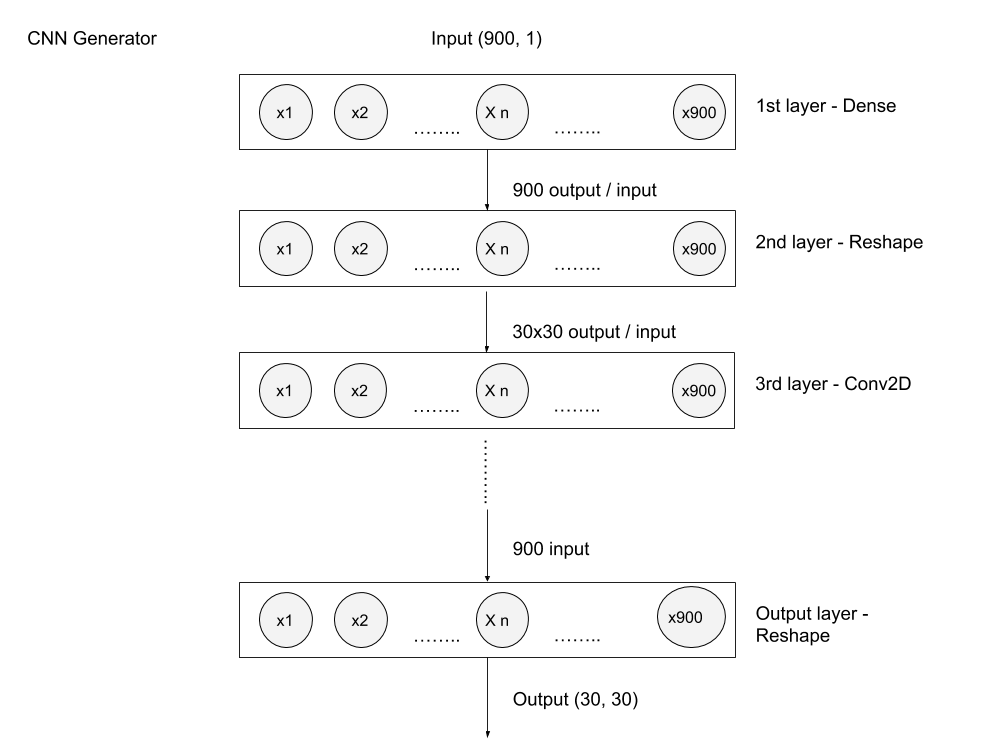
\includegraphics[width=.8\linewidth]{../images/graphs/CNN_generator.png}
\caption{Απεικόνιση των επιπέδων του CNN Generator}
\label{fig:fig}
\end{figure}


\subsection{Αρχιτεκτονική Discriminator}
Αντίστοιχα με το Discriminator μοντέλο του Dense δικτύου, έτσι και του CNN είναι πολύ πιο μικρό σε σχέση με τον Generator. Παρατηρούμε ομοιότητες με το μοντέλο του Generator του CNN αλλά και με το Discriminator του Dense.

\begin{verbatim}
Conv2D(32, 3, padding='same', strides=2, input_shape=self.dungeon_shape)
LeakyReLU(0.2)
Dropout(0.3)

Conv2D(64, 3, padding='same', strides=1)
LeakyReLU(0.2)
Dropout(0.3)

Flatten()
Dense(1, activation="sigmoid")

\end{verbatim}

\begin{figure}[H]
\centering
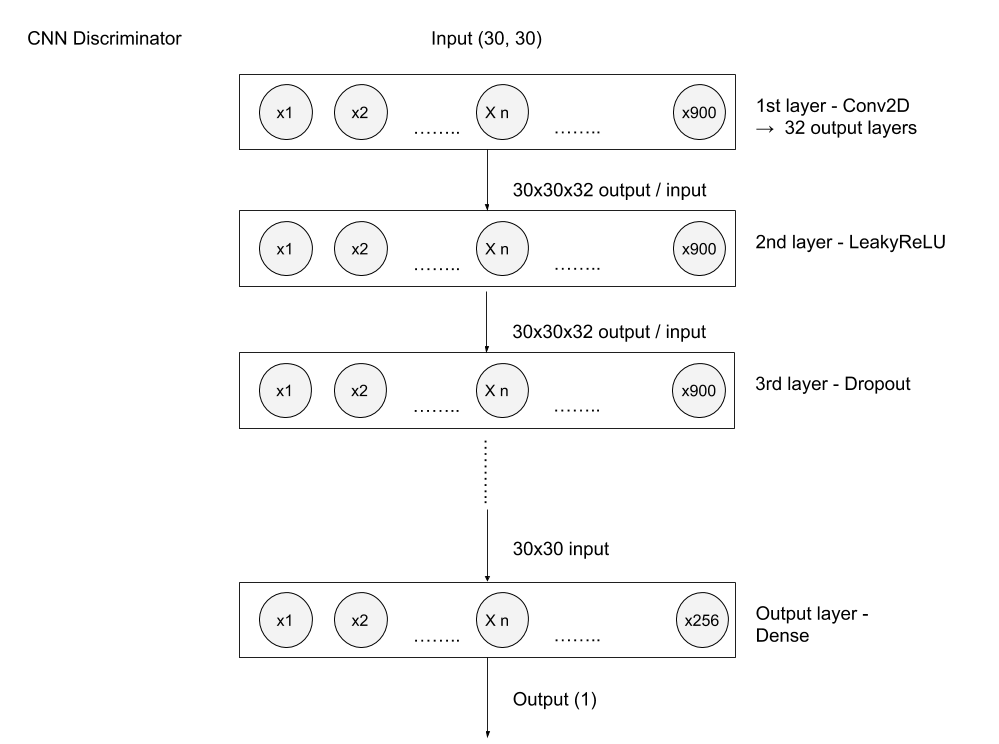
\includegraphics[width=.8\linewidth]{../images/graphs/CNN_discriminator.png}
\caption{Απεικόνιση των επιπέδων του CNN Discriminator}
\label{fig:fig}
\end{figure}

\section{Εκπαίδευση GAN}
Για την εκπαίδευση των δύο GAN χρησιμοποιήθηκε το ίδιο dataset όπως αυτό δημιουργήθηκε από την υλοποίηση του PCG. Το dataset αποτελείται από 114 αρχεία όπου το κάθε αρχείο αντιστοιχεί σε ένα επίπεδο. Πριν ξεκινήσει η διαδικασία την εκπαίδευσης, φορτώνονται όλα τα επίπεδα στην μνήμη και περνάνε από το στάδιο της προ επεξεργασίας για να έρθουν σε μορφή που να μπορούν να επεξεργαστούν τα δύο μοντέλα GAN.
\par
Η διαδικασία της εκπαίδευσης είναι κοινή και για τα δύο μοντέλα.


\begin{figure}[H]
\centering
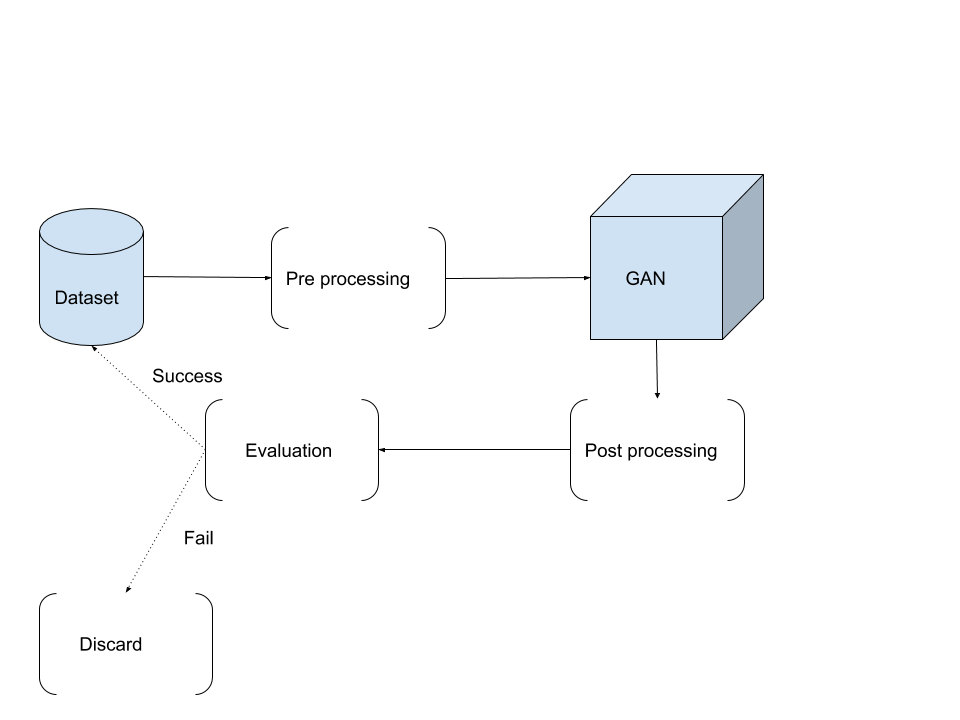
\includegraphics[width=.8\linewidth]{../images/graphs/Abstract_functionality.png}
\caption{Αναπαράσταση εκπαίδευσης ενός μοντέλου GAN}
\label{fig:fig}
\end{figure}

\subsection{Μεταβλητές εκπαίδευσης}
Κατά την δημιουργία του μοντέλου ορίζονται μεταβλητές που θα χρησιμοποιηθούν στο στάδιο της εκπαίδευσης. Όλες οι μεταβλητές έχουν προ ρυθμισμένες τιμές οι οποίες βγήκαν μέσα από δοκιμές. Μερικές από τις πιο σημαντικές είναι:

\begin{description}
\item[$\bullet$ epochs] Θετικός ακέραιος αριθμός που ορίζει τον αριθμό των εποχών που θα επαναληφθεί η εκπαίδευση. Η προτεινόμενη τιμή του για αυτή την υλοποίηση είναι 10000.
\item[$\bullet$ batch\_size] Θετικός ακέραιος αριθμός που ορίζει τον αριθμό των δειγμάτων που θα δίνονται σε κάθε εποχή για εκπαίδευση. Εάν το batch\_size είναι μικρότερο του μεγέθους του dataset, τα δείγματα που θα συμμετέχουν στην εκπαίδευση επιλέγονται τυχαία με δειγματοληψία σε κάθε εποχή και χωρίς επανατοποθέτηση. Στην περίπτωση που το batch\_size είναι μεγαλύτερο του μεγέθους του dataset, ορίζετε ως batch\_size το μέγεθος του dataset. Η προτεινόμενη τιμή του για αυτή την υλοποίηση είναι 64.
\item[$\bullet$ sample] Θετικός ακέραιος αριθμός που ορίζει το διάστημα ανάμεσα στις εποχές που λαμβάνουμε ένα δείγμα επιπέδου από το μοντέλο σε εκείνο το στάδιο της εκπαίδευσης. Αυτή η μεταβλητή ορίστηκε για να μπορούμε να παρακολουθούμε την πρόοδο του δικτύου όσο εκπαιδεύεται. Η προτεινόμενη τιμή του για αυτή την υλοποίηση είναι 1000.
\item[$\bullet$ train\_discriminator] Μία δυαδική μεταβλητή που ορίζει εάν θα πρέπει να εκπαιδεύσουμε και το δίκτυο του Discriminator. Σε περίπτωση που οριστεί να μην εκπαιδευτεί, το δίκτυο του Discriminator δεν θα πραγματοποιεί διόρθωση βαρών ανά τις εποχές της εκπαίδευσης. Παρατηρήθηκαν καλύτερα αποτελέσματα όταν εκπαιδεύαμε και το δίκτυο του Discriminator. Η προτεινόμενη τιμή του για αυτή την υλοποίηση είναι \textit{True}.
\end{description}

\subsection{Είσοδος εκπαίδευσης Generator}
Για την εκπαίδευση του Generator δίνουμε ως είσοδο στο δίκτυο, δύο πίνακες που περιέχουν ίδιο αριθμό δειγμάτων. Το κάθε δείγμα έχει την μορφή προ επεξεργασμένου επιπέδου. Ο αριθμός των δειγμάτων ορίζετε από το batch\_size. O ένας πίνακας περιέχει δείγματα από το dataset ενώ ο άλλος πίνακας περιέχει \textit{θόρυβο}, δηλαδή τυχαία δημιουργημένα δείγματα που έχουν τιμές στο διάστημα που ορίσαμε για τα δείγματα των επιπέδων. 
\par
Τα στοιχεία των δύο πινάκων αντιστοιχίζονται ένα προς ένα καθώς ως στόχο το δίκτυο έχει να μετατρέψει τα δείγματα του θορύβου στα αντίστοιχα δείγματα του dataset μέσα από τις μετατροπές που θα εφαρμόσει. Το τελικό αποτέλεσμα συγκρίνετε με το επιθυμητό αποτέλεσμα, το επίπεδο από το dataset, και διορθώνονται τα βάρη των επιπέδων αντίστοιχα.

\subsection{Λειτουργία Generator}
Για την λειτουργία του Generator, εκτός του σταδίου της εκπαίδευσης, πρέπει να του δώσουμε ως είσοδο ένα δείγμα θορύβου για να δημιουργήσει ένα δείγμα επιπέδου.

\subsection{Είσοδος εκπαίδευσης Discriminator}
Για την εκπαίδευση του Discriminator δίνουμε ως είσοδο έναν πίνακα και ένα διάνυσμα. Ο πίνακας περιέχει τα δείγματα που θέλουμε να αξιολογήσει ως "τεχνητά" από τον Generator ή "πραγματικά" από το dataset. Το διάνυσμα έχει δυαδικές τιμές που δηλώνουν την πραγματική προέλευση του κάθε δείγματος με τις τιμές 0 και 1.
\par
Για να εκπαιδευτεί ο Discriminator παίρνει ως είσοδο τα επίπεδα και ελέγχει την έξοδο του εάν ταιριάζει με την αντίστοιχη τιμή για αυτό το επίπεδο με το διάνυσμα των πραγματικών τιμών. Ομοίως διορθώνει τα βάρη του στις περιπτώσεις λάθους εάν έχουμε ενεργοποιήσει την μεταβλητή train\_discriminator.

\section{Εκπαίδευση μοντέλου}
\par
Η εκπαίδευση του GAN μοντέλου, γίνεται σε δύο στάδια. Στο πρώτο στάδιο εκπαιδεύεται το μοντέλο του Generator με το υπάρχον dataset χωρίς την ανατροφοδότηση από το μοντέλο του Discriminator. Όπως φαίνεται και από τον πίνακα 4.1, το μοντέλο του Generator με τις ορισμένες παραμέτρους μπορεί να φτάσει μέχρι ένα συγκεκριμένο ποσοστό ακρίβειας και σφάλματος χωρίς να βελτιώνετε παραπάνω.
\par
Στο δεύτερο στάδιο, εκπαιδεύουμε και τα δύο μοντέλα, τον Generator και τον Discriminator μαζί σε συνεργασία και όπως φαίνεται από τον πίνακα 4.2 πετυχαίνουμε πολύ καλύτερα επίπεδα ακρίβειας και χαμηλότερο σφάλμα, όπως επιβεβαιώνουν και οι εικόνες από τα επίπεδα που παράχθηκαν από το δεύτερο στάδιο της εκπαίδευσης.


\section{Αποτελέσματα μοντέλου CNN}

\subsection{Αποτελέσματα του Generator του CNN δικτύου}
\begin{figure}[H]
\begin{subfigure}{.5\textwidth}
  \centering
  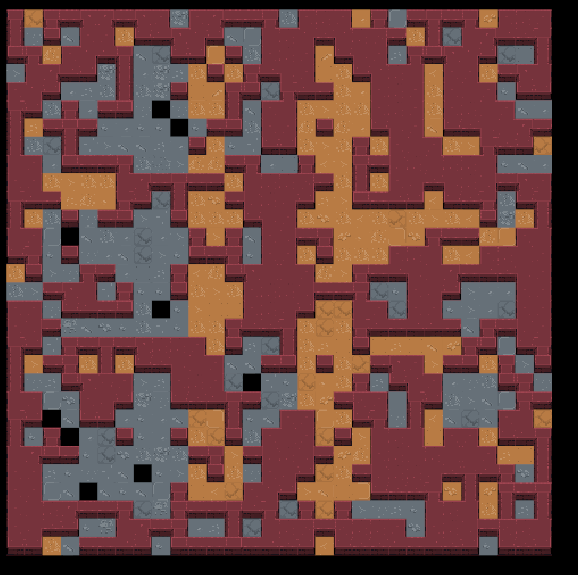
\includegraphics[width=.8\linewidth]{../images/result_images/cnn-gan/generator_1000.png}
  \caption{Επίπεδο μετά από 1000 εποχές}
  \label{fig:sfig1}
\end{subfigure}%
\begin{subfigure}{.5\textwidth}
  \centering
  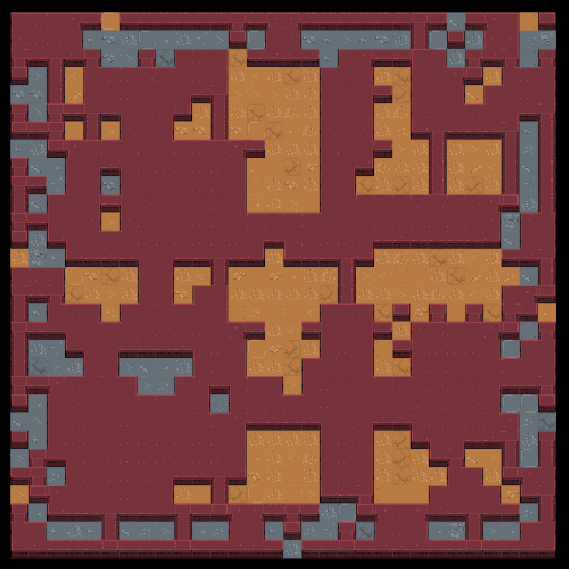
\includegraphics[width=.8\linewidth]{../images/result_images/cnn-gan/generator_3000.png}
  \caption{Επίπεδο μετά από 3000 εποχές}
  \label{fig:sfig2}
\end{subfigure}
\begin{subfigure}{.5\textwidth}
  \centering
  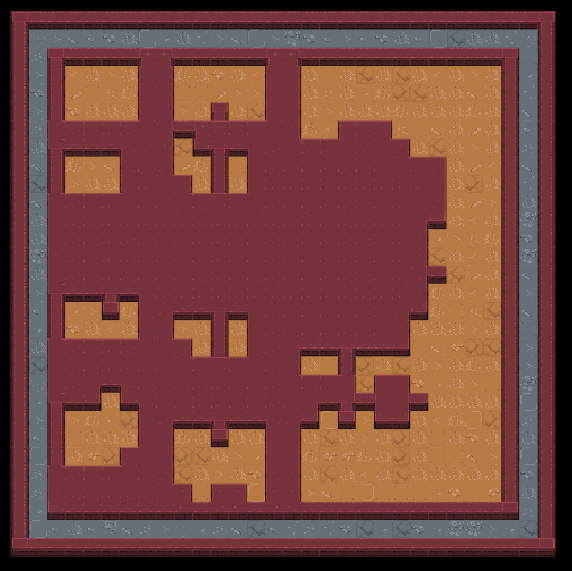
\includegraphics[width=.8\linewidth]{../images/result_images/cnn-gan/generator_7000.png}
  \caption{Επίπεδο μετά από 7000 εποχές}
  \label{fig:sfig2}
\end{subfigure}
\begin{subfigure}{.5\textwidth}
  \centering
  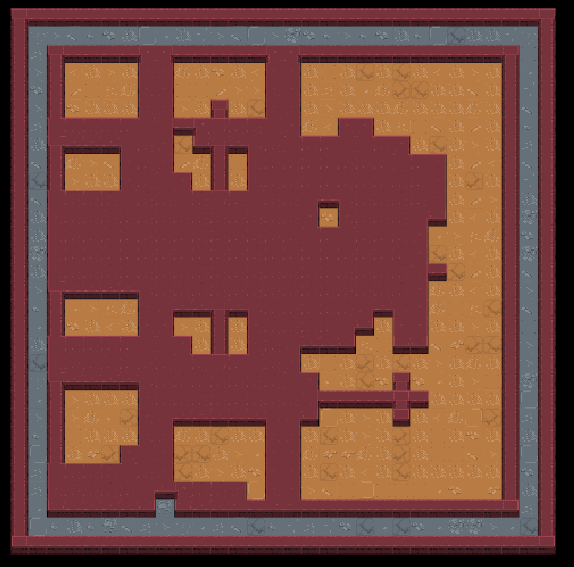
\includegraphics[width=.8\linewidth]{../images/result_images/cnn-gan/generator_10000.png}
  \caption{Επίπεδο μετά από 10000 εποχές}
  \label{fig:sfig2}
\end{subfigure}
\caption{Επίπεδα που δημιούργησε κατά την εκπαίδευση το μοντέλο του Generator χωρίς σύνδεση με το μοντέλο του Discriminator, χωρίς προσθήκη θορύβου στα δεδομένα εισόδου.}
\label{fig:fig}
\end{figure}

\begin{center}
\begin{tabular}{|l|l|l|}
\hline
\textbf{Εποχή} & \textbf{Σφάλμα} & \textbf{Ακρίβεια} \\ \hline
1000		   & 1.112154        & 0.35\%            \\ \hline
2000		   & 0.814016        & 0.40\%            \\ \hline
3000		   & 0.572094        & 0.48\%            \\ \hline
4000		   & 0.439945        & 0.56\%            \\ \hline
5000		   & 0.378878        & 0.62\%            \\ \hline
6000		   & 0.329374        & 0.67\%            \\ \hline
7000		   & 0.320769        & 0.67\%            \\ \hline
8000		   & 0.306775        & 0.67\%            \\ \hline
9000		   & 0.311993        & 0.67\%            \\ \hline
10000		   & 0.316760        & 0.67\%            \\ \hline
\end{tabular}
\end{center}
\captionof{table}{Μετρήσεις σφάλματος και ακρίβειας για το μοντέλο του Generator} \label{tab:title}

\subsection{Αποτελέσματα του Generator και του Discriminator του CNN δικτύου}
\begin{figure}[H]
\begin{subfigure}{.5\textwidth}
  \centering
  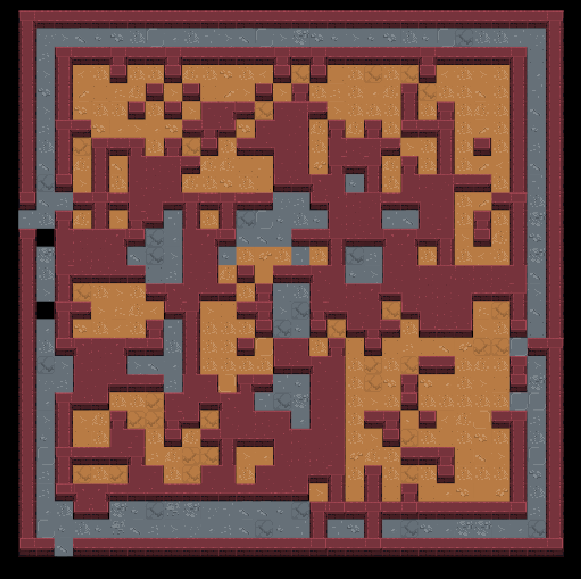
\includegraphics[width=.8\linewidth]{../images/result_images/cnn-gan/combined_1000.png}
  \caption{Επίπεδο μετά από 1000 εποχές}
  \label{fig:sfig1}
\end{subfigure}%
\begin{subfigure}{.5\textwidth}
  \centering
  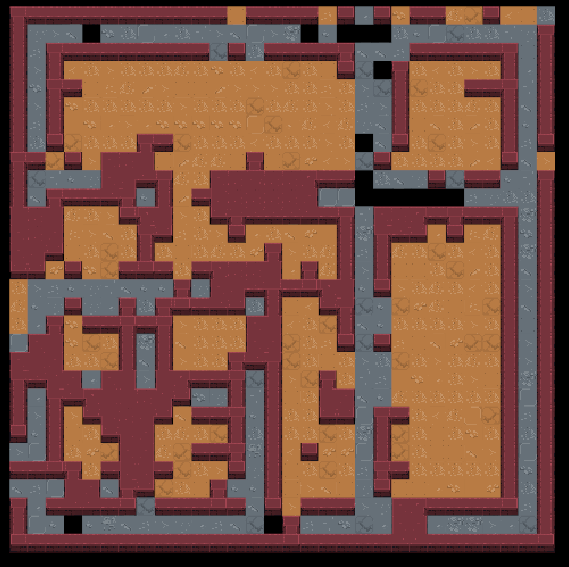
\includegraphics[width=.8\linewidth]{../images/result_images/cnn-gan/combined_3000.png}
  \caption{Επίπεδο μετά από 3000 εποχές}
  \label{fig:sfig2}
\end{subfigure}
\begin{subfigure}{.5\textwidth}
  \centering
  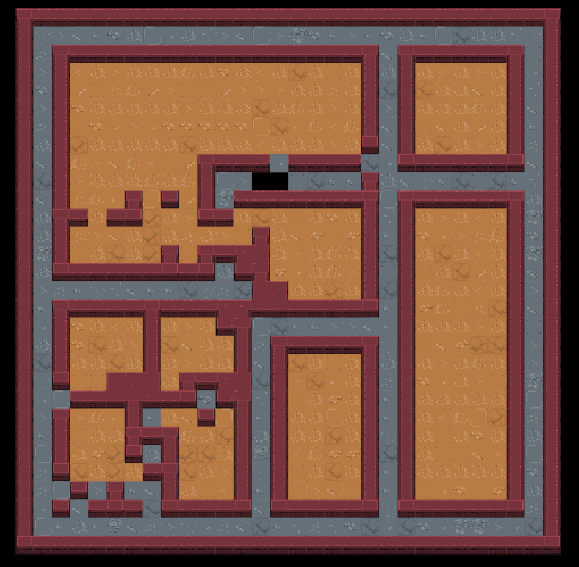
\includegraphics[width=.8\linewidth]{../images/result_images/cnn-gan/combined_7000.png}
  \caption{Επίπεδο μετά από 7000 εποχές}
  \label{fig:sfig2}
\end{subfigure}
\begin{subfigure}{.5\textwidth}
  \centering
  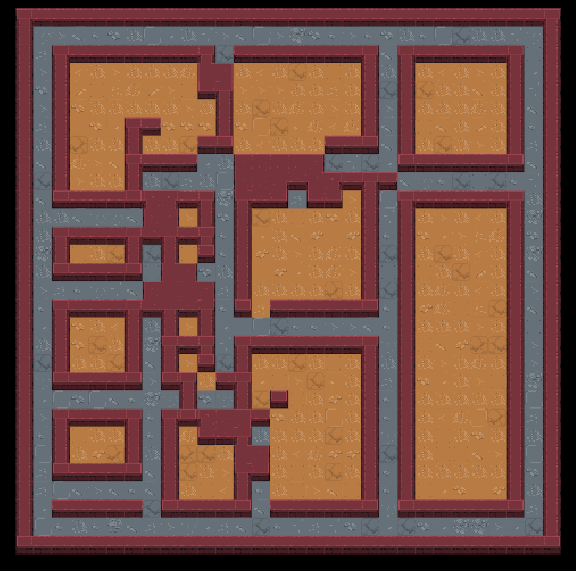
\includegraphics[width=.8\linewidth]{../images/result_images/cnn-gan/combined_10000.png}
  \caption{Επίπεδο μετά από 10000 εποχές}
  \label{fig:sfig2}
\end{subfigure}
\caption{Επίπεδα που δημιούργησε κατά την εκπαίδευση το μοντέλο του Generator με το μοντέλο του Discriminator}
\label{fig:fig}
\end{figure}

\begin{center}
\begin{tabular}{|l|l|l|}
\hline
\textbf{Εποχή} & \textbf{Σφάλμα} & \textbf{Ακρίβεια} \\ \hline
1000		   & 0.239428        & 0.67\%            \\ \hline
2000		   & 0.225229        & 0.73\%            \\ \hline
3000		   & 0.179896        & 0.89\%            \\ \hline
4000		   & 0.190461        & 0.84\%            \\ \hline
5000		   & 0.181195        & 0.91\%            \\ \hline
6000		   & 0.181408        & 0.92\%            \\ \hline
7000		   & 0.181004        & 0.91\%            \\ \hline
8000		   & 0.191332        & 0.86\%            \\ \hline
9000		   & 0.185095        & 0.89\%            \\ \hline
10000		   & 0.190194        & 0.84\%            \\ \hline
\end{tabular}
\end{center}
\captionof{table}{Μετρήσεις σφάλματος και ακρίβειας για το μοντέλο του Generator και του Discriminator} \label{tab:title}

\section{Αποτελέσματα μοντέλου Dense}

\subsection{Αποτελέσματα του Generator του Dense δικτύου}
\begin{figure}[H]
\begin{subfigure}{.5\textwidth}
  \centering
  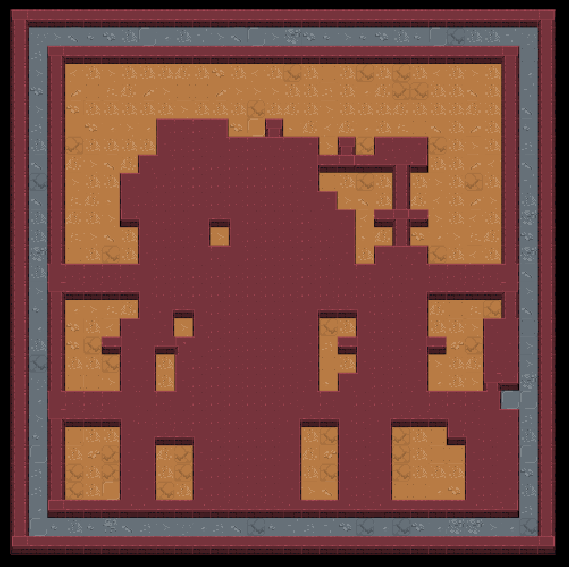
\includegraphics[width=.8\linewidth]{../images/result_images/dense-gan/generator_1000.png}
  \caption{Επίπεδο μετά από 1000 εποχές}
  \label{fig:sfig1}
\end{subfigure}%
\begin{subfigure}{.5\textwidth}
  \centering
  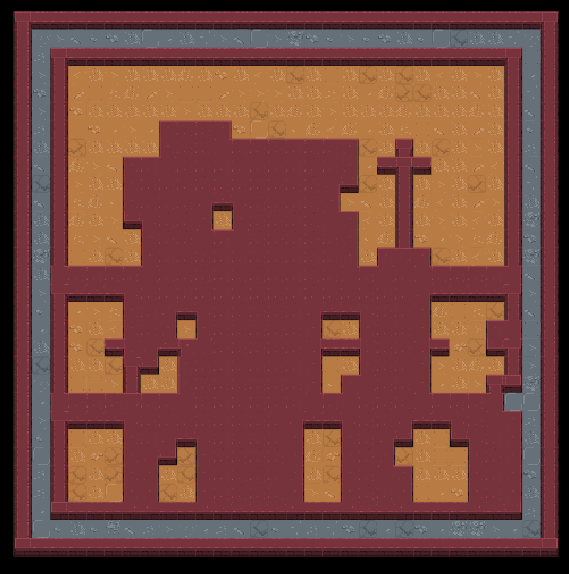
\includegraphics[width=.8\linewidth]{../images/result_images/dense-gan/generator_3000.png}
  \caption{Επίπεδο μετά από 3000 εποχές}
  \label{fig:sfig2}
\end{subfigure}
\begin{subfigure}{.5\textwidth}
  \centering
  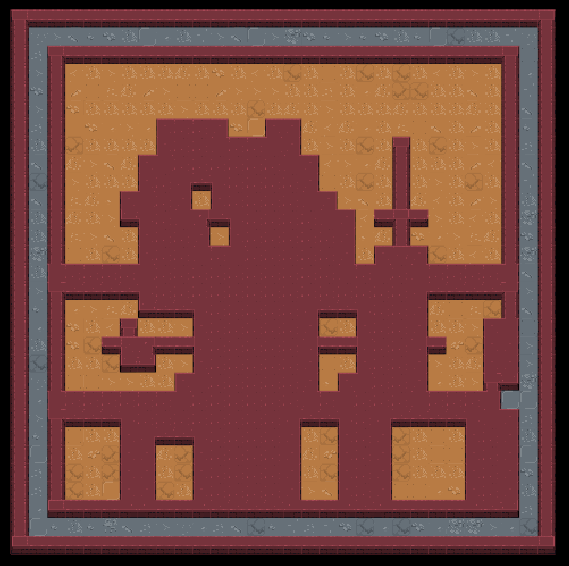
\includegraphics[width=.8\linewidth]{../images/result_images/dense-gan/generator_7000.png}
  \caption{Επίπεδο μετά από 7000 εποχές}
  \label{fig:sfig2}
\end{subfigure}
\begin{subfigure}{.5\textwidth}
  \centering
  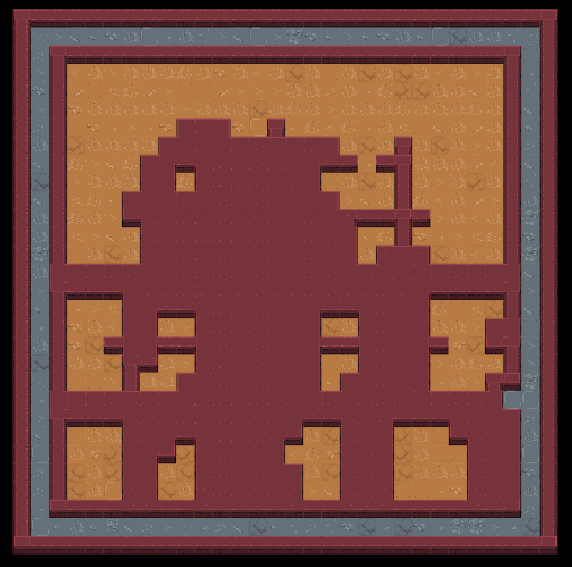
\includegraphics[width=.8\linewidth]{../images/result_images/dense-gan/generator_10000.png}
  \caption{Επίπεδο μετά από 10000 εποχές}
  \label{fig:sfig2}
\end{subfigure}
\caption{Επίπεδα που δημιούργησε κατά την εκπαίδευση το μοντέλο του Generator χωρίς σύνδεση με το μοντέλο του Discriminator.}
\label{fig:fig}
\end{figure}

\subsection{Αποτελέσματα του Generator και του Discriminator του Dense δικτύου}
\begin{figure}[H]
\begin{subfigure}{.5\textwidth}
  \centering
  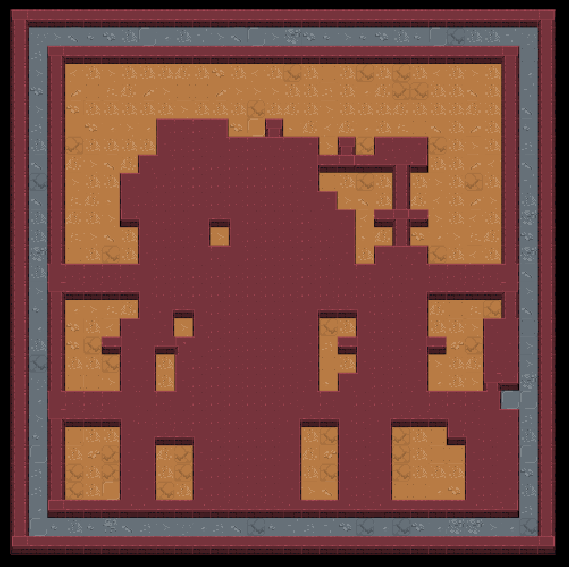
\includegraphics[width=.8\linewidth]{../images/result_images/dense-gan/generator_1000.png}
  \caption{Επίπεδο μετά από 1000 εποχές}
  \label{fig:sfig1}
\end{subfigure}%
\begin{subfigure}{.5\textwidth}
  \centering
  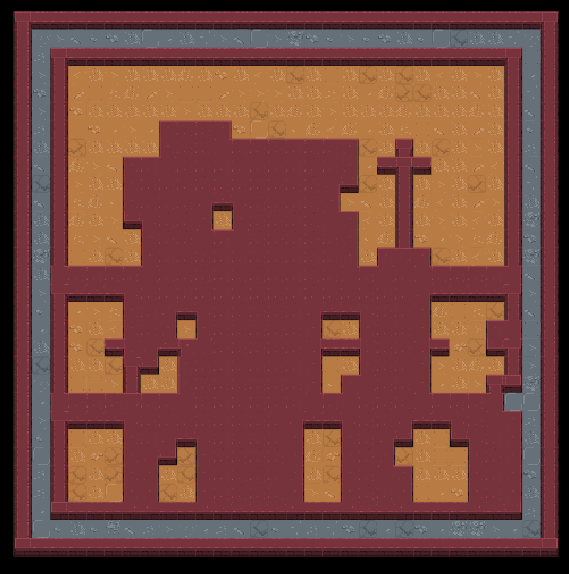
\includegraphics[width=.8\linewidth]{../images/result_images/dense-gan/generator_3000.png}
  \caption{Επίπεδο μετά από 3000 εποχές}
  \label{fig:sfig2}
\end{subfigure}
\begin{subfigure}{.5\textwidth}
  \centering
  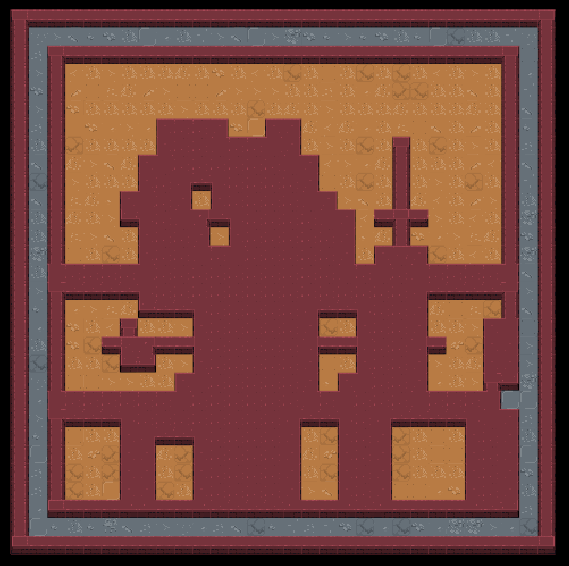
\includegraphics[width=.8\linewidth]{../images/result_images/dense-gan/generator_7000.png}
  \caption{Επίπεδο μετά από 7000 εποχές}
  \label{fig:sfig2}
\end{subfigure}
\begin{subfigure}{.5\textwidth}
  \centering
  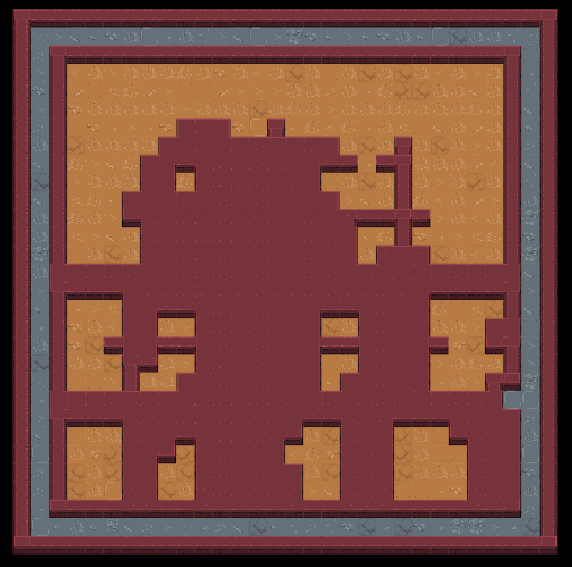
\includegraphics[width=.8\linewidth]{../images/result_images/dense-gan/generator_10000.png}
  \caption{Επίπεδο μετά από 10000 εποχές}
  \label{fig:sfig2}
\end{subfigure}
\caption{Επίπεδα που δημιούργησε κατά την εκπαίδευση το μοντέλο του Generator με το μοντέλο του Discriminator.}
\label{fig:fig}
\end{figure}

\par
Κατά την εκπαίδευση του Dense μοντέλου, όλες οι μετρήσεις που παράχθηκαν από το σύστημα ήταν λάθος το οποίο το αποδίδουμε σε λάθος επιλογή μετρικών (mean square error, accuracy) για το είδος της εφαρμογής και της αρχιτεκτονικής αυτού του δικτύου. Τα αποτελέσματα που παράχθηκαν από το δίκτυο με οπτική αξιολόγηση φαίνεται να βελτιώνονται ως ένα βαθμό αλλά να "κολλάνε" σε ένα συγκεκριμένο μοτίβο.
